\documentclass[11pt,aspectratio=1610]{beamer}
\usetheme{default}
\usepackage[utf8]{inputenc}
\usepackage[T1]{fontenc}
\usepackage{hyperref}
\usepackage{graphicx}
% \usepackage{subfig}
\usepackage[font=scriptsize]{caption}
\usepackage[font=scriptsize]{subcaption}
\captionsetup[subfigure]{position=top}

\usepackage[
    backend=biber,
    style=numeric,
    natbib=true,
    url=false, 
    sorting=none,
    doi=true,
    eprint=false
]{biblatex}
\addbibresource{Biblio.bib}

\usepackage[tensorialbold]{userCommands}
\usepackage[babel=true,kerning=true]{microtype}
\usepackage{amsmath}
\usepackage{amsfonts}
\usepackage{amssymb}
\usepackage{pifont}
\usepackage{mathrsfs}
\usepackage{graphicx}
\usepackage{wasysym}

\usepackage{fancybox}
\usepackage{textcomp}
\usepackage{multicol}
\usepackage{xcolor}
\usepackage{lmodern}
\usepackage{tkz-kiviat}
\RequirePackage{tikz}
\usetikzlibrary{patterns} 
\usetikzlibrary{shapes}
\usetikzlibrary{snakes}
\usetikzlibrary{pgfplots.groupplots}
\usetikzlibrary{spy,backgrounds}
\usetikzlibrary{decorations.markings}
\usetikzlibrary{arrows.meta}

\usepackage{pgfplots}
% \usepackage{pgfplotsthemetol}
\pgfplotsset{compat=newest,
  grid=both,
  every axis/.append style={font=\scriptsize},
  tick label style={font=\scriptsize},
  label style={font=\scriptsize},
  title style={font=\scriptsize},
  legend style={font=\footnotesize},
  legend cell align={left},
  yticklabel style={/pgf/number format/fixed},
  % define user colormap
  colormap={tol}{[1cm] rgb255(0cm)=(120,28,129) rgb255(1cm)=(63,96,174) rgb255(2cm)=(83,158,182) rgb255(3cm)=(109,179,136) rgb255(4cm)=(202,184,67) rgb255(5cm)=(231,133,50) rgb255(6cm)=(217,33,32)}
}

\newcommand{\xmark}{\color{Red}\ding{55}}
\newcommand{\cmark}{\color{Green}\ding{51}}

%% User colors
\definecolor{Purple}{RGB}{120,28,129}
\definecolor{Blue}{RGB}{63,96,174}
\definecolor{Duck}{RGB}{83,158,182}
\definecolor{Green}{RGB}{109,179,136}
\definecolor{Yellow}{RGB}{202,184,67}
\definecolor{Orange}{RGB}{231,133,50}
\definecolor{Red}{RGB}{217,33,32}

\usefonttheme{professionalfonts}

\usetheme[progressbar=foot,
subsectionpage=none,
sectionpage=progressbar,
block=transparent%fill
]{metropolis}

%\useoutertheme{Headinfoline}
%\setbeamertemplate{section in toc}{{\inserttocsectionnumber.}~\inserttocsection    \vspace{-.05\baselineskip}}
% \setbeamertemplate{subsection in toc}{{\inserttocsubsectionnumber.}~\inserttocsubsection    \vspace{-.1\baselineskip}}

\setbeamerfont{section in toc}{size=\normalsize,series=\bfseries}
\setbeamerfont{subsection in toc}{size=\footnotesize}
    
%% CHANGE COLOR SETTINGS
\definecolor{mDarkBrown}{HTML}{604c38}
\definecolor{mDarkTeal}{HTML}{23373b}
\definecolor{mLightBrown}{HTML}{EB811B}
\definecolor{mLightGreen}{HTML}{14B03D}
\definecolor{CNBlue}{RGB}{16,38,72}
\definecolor{CNYellow}{RGB}{250,182,0}

%% fg= ; bg= background 
%\setbeamercolor{normal text}{ fg= CNBlue!90 , bg= black!2 }
%\setbeamercolor{alerted text}{ fg=mDarkTeal  }
%\setbeamercolor{exemple text}{ fg=mDarkTeal  }



\setbeamerfont{bibliography entry author}{size=\scriptsize,series=\normalfont}
\setbeamerfont{bibliography entry title}{size=\scriptsize,series=\bfseries}
\setbeamerfont{bibliography entry location}{size=\scriptsize, series=\normalfont}
\setbeamerfont{standout}{size=\Large,series=\bfseries}
%%%%%%%%%%caracterisation du document %---------------------------------------------------------------------
\hypersetup{
	pdftitle    = {Formulation of the DGMPM},
	pdfsubject  = {Ph.D thesis defense- December 2018},
	linkcolor    = red,
	pdfauthor   = {Adrien Renaud},
	pdfkeywords = {numerical simulation, hyperbolic problems, discontinuous Galerkin}
	colorlinks=true,
	linkcolor=black,
	citecolor=blue,
	urlcolor=blue
}



%%-------------- Construction de la page de presentation -------------------------------------------------------
\title[Réunion Modus3d -- Avril]
{\Large\bf  {Projet Modus3d -- Réunion d'Avril }}

\date[]{}
%\author{A. Renaud \\ Supervisors: T. Heuz\'e, L. Stainier} 


%------------------------------------------------------------------------

\setbeamertemplate{bibliography item}{\insertbiblabel}

%% Baptist's beamer clock

\newcommand{\myBeamerClock}[2]{
  % #1 is the radius of the clock
  % #2 is the vertical shift for inline placement
  % #3 is the number of current frame
  % #4 is the total number of frames
  \tikz[baseline=#2]{
    \filldraw (0,0) -- (0,#1) arc (90:(90-(\insertframenumber/\inserttotalframenumber)*360):#1);
    \draw (0,0) circle (#1);
  }
}

\newcommand{\footnoteCite}[1]{
  {\tiny 
  \begin{flushleft}
    \foreach \x in {#1}{\cite{\x}  \fullcite{\x}\\}
  \end{flushleft}
}
}
  

%% OR with baptiste's clock
\defbeamertemplate*{footline}{mytheme}{%
  \usebeamerfont{page number in head/foot}\begin{beamercolorbox}[sep=1.em]{} \hfill  \insertframenumber{} \myBeamerClock{1ex}{-1ex} 
 \end{beamercolorbox}
}


\pgfplotsset{select coords between index/.style 2 args={
    x filter/.code={
        \ifnum\coordindex<#1\def\pgfmathresult{}\fi
        \ifnum\coordindex>#2\def\pgfmathresult{}\fi
    }
  }}



\begin{document}

\begin{frame}[plain]
  \maketitle
\end{frame}

\begin{frame}[plain]
  \frametitle{Ordre du jour}\tableofcontents[hideallsubsections]
\end{frame}



\AtBeginSection[]{%
  \begin{frame}[plain,]\frametitle{Ordre du jour}\tableofcontents[currentsection,hideallsubsections]\end{frame}}

\section{Générateurs de microstructures}

\begin{frame}{Neper}
  \begin{block}{Génération à partir de propriétés morphologiques \cite{Neper,Neper_Bimodal}}
    \begin{itemize}
    \item Tessellation de Laguerre ou Voronoi
    \item Densités de probabilité (taille de grain; sphéricité etc.)
    \end{itemize}
    \begin{columns}
      \begin{column}{0.45\linewidth}
        \begin{center}
          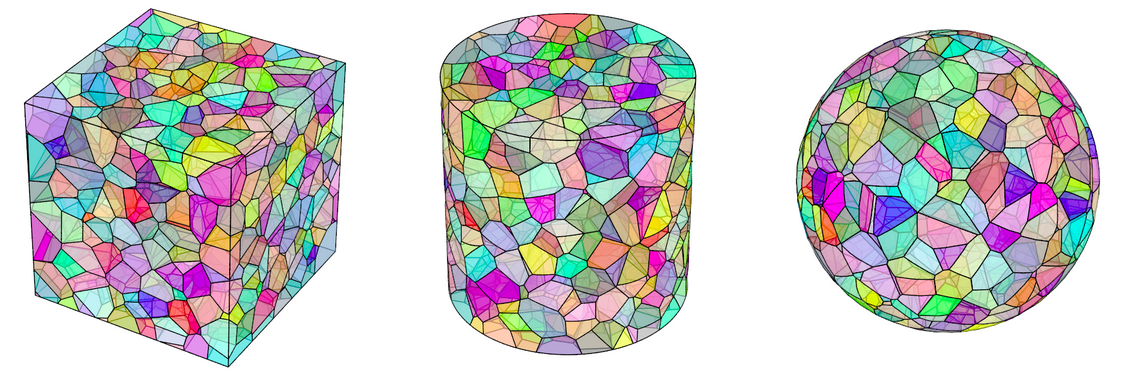
\includegraphics[width=0.95\linewidth]{pngFigures/neper_volumes.png} \\
          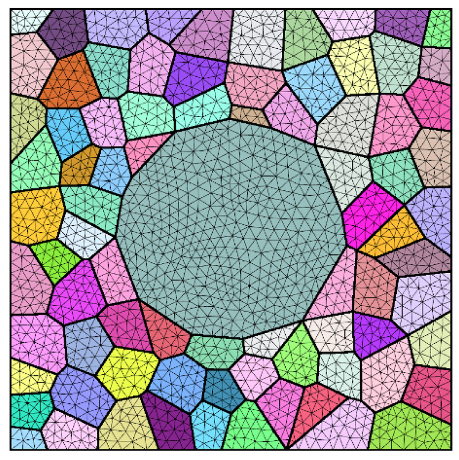
\includegraphics[width=0.3\textwidth]{pngFigures/neper_bimodal}
        \end{center}
      \end{column}
      \begin{column}{0.25\linewidth}
        \centering
        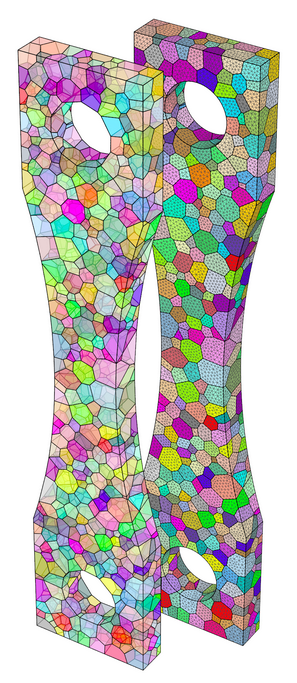
\includegraphics[width=0.55\linewidth]{pngFigures/neper_bielle.png}
      \end{column}
      \begin{column}{0.25\linewidth}
        \centering
        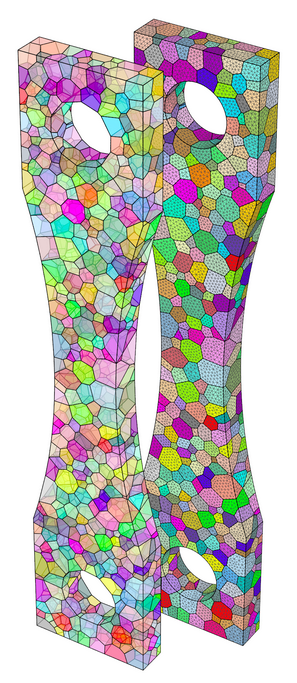
\includegraphics[width=0.55\linewidth]{pngFigures/neper_bielle.png}
        \footnotesize{anisotrope}
      \end{column}
    \end{columns}
    \begin{itemize}
    \item Maillage volumique "régularisé" (\textsc{GMSH})
    \end{itemize}
  \end{block}

  \vspace{-0.4 cm}
  \footnoteCite{Neper,Neper_Bimodal}
\end{frame}
%% Parler de Neper

\begin{frame}{Dream3D}
  \begin{block}{Génération à partir de propriétés morphologiques \cite{Dream3D}}
    \begin{itemize}
    \item Assemblage de grains jusqu'à remplissage dans un cube ($\rightarrow$ vides)
    \item Grains éllipsoïdaux, octahédriques ou cylindriques
    \end{itemize}
    \centering
    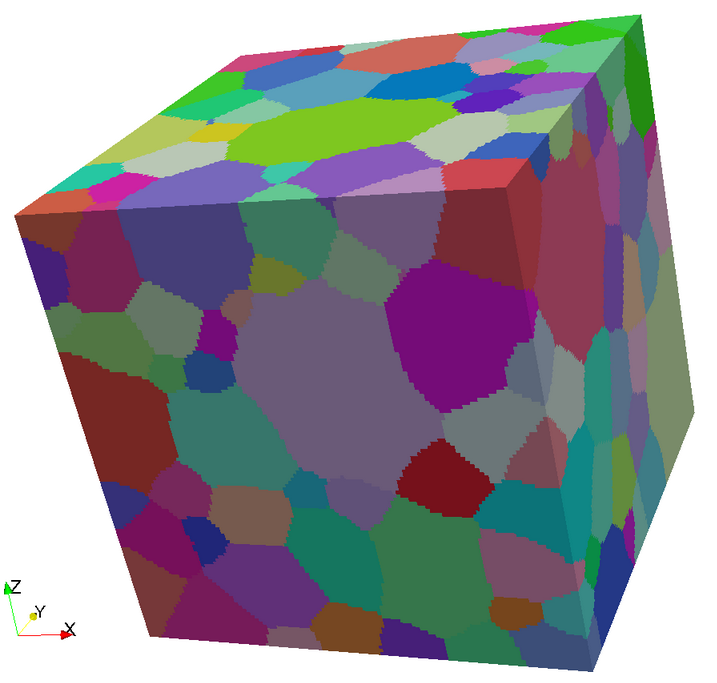
\includegraphics[scale=0.10]{pngFigures/dream3d_cube.png} \qquad\qquad
    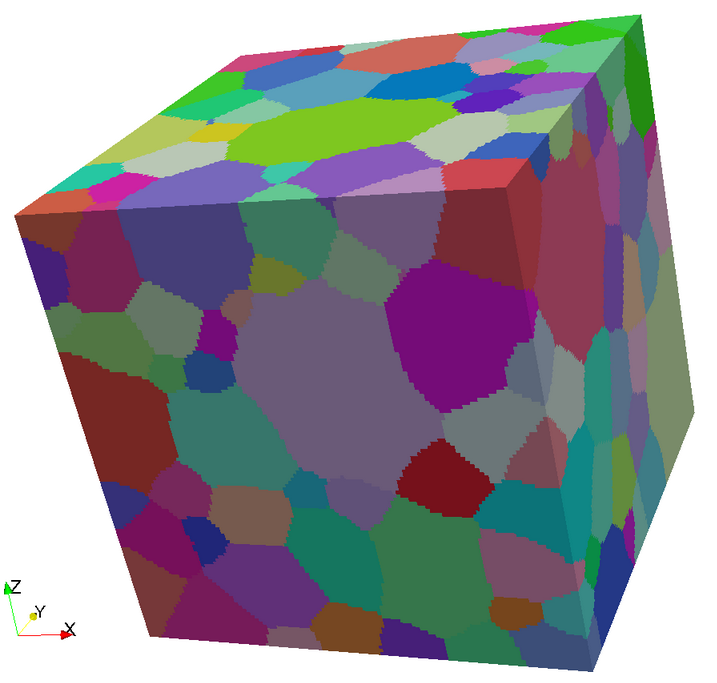
\includegraphics[scale=0.10]{pngFigures/dream3d_cube.png} (maillage)
  \end{block}
  \begin{block}{\alert{Reconstruction EBSD}}
    \begin{itemize}
    \item Attribution d'orientations à des voxels
    \end{itemize}
  \end{block}
  \begin{block}{Maillage surfacique}
    \begin{itemize}
    \item Maillage surfacique des interfaces "voxelisées" (lissage possible)
    \end{itemize}
  \end{block}
  \vspace{-0.4 cm}
  \footnoteCite{Dream3D}
\end{frame}
%% Parler de Dream3D

\begin{frame}{Comparatif}
  \centering
  \begin{tabular}[h]{l|c|c}
    & Neper  & Dream3D \\
    \hline
    \hline
    Génération  &   \color{Green}{Voronoi}          & \color{Orange} Assemblage \\
                &   \color{Green}2D -- 3D    & \color{Orange} 3D \\
                &   \color{Green}Domaine convexe    & \color{Orange} Domaine cubique \\
    \hline
    Reconstruction EBSD  &   \color{Red}{Non}       & \color{Green} Oui \\
    \hline
    Sortie      &   \color{Green} Points + Connectivités   & \color{Red} Collection de Voxels \\
    \hline                  
  \end{tabular}
  \pause
  \vspace{1cm}
  \begin{block}{$\Rightarrow$ Neper retenu pour "couplage" avec oofe}
    
  \end{block}

\end{frame}

\section{Couplage avec OOFE}
\begin{frame}{Calcul sur microstructures Neper}
  \begin{block}{Microstructures 2D}
    \begin{itemize}
    \item domaine rectangulaire : fait
    \item domaine circulaire : en cours
    \end{itemize}
  \end{block}
  \begin{block}{Microstructures 3D}
    \begin{itemize}
    \item[] A faire 
    \end{itemize}
  \end{block}
\end{frame}
%% C'est implémenté en 2D

\section{}



%% Ca ne requiert pas de lecture de données EBSD
\section{Reste à faire en 2D}

\section{Reste à faire en 3D}

%% Mais si on veut le faire, on va surement devoir utiliser dream3D et donc travailler sur le dialogue avec OOFE
\section{Lecture de reconstruction EBSD}


\end{document}

%%% Local Variables:
%%% mode: latex
%%% TeX-master: t
%%% End:
